%%%%%%%%%%%%%%%%%%%%%%%%%%%%%%%%%%%%%%%%%
% Beamer Presentation
% LaTeX Template
% Version 1.0 (10/11/12)
%
% This template has been downloaded from:
% http://www.LaTeXTemplates.com
%
% License:
% CC BY-NC-SA 3.0 (http://creativecommons.org/licenses/by-nc-sa/3.0/)
%
%%%%%%%%%%%%%%%%%%%%%%%%%%%%%%%%%%%%%%%%%

%----------------------------------------------------------------------------------------
%	PACKAGES AND THEMES
%----------------------------------------------------------------------------------------

\documentclass{beamer}
\usepackage{amsmath,amsthm,amssymb,amsfonts,graphicx} % The standard ams packages used very commonly
\usepackage{hyperref} % Used to make links or other things like that relating to the internet.
\usepackage[backend=bibtex, style=numeric]{biblatex}
% \usepackage{xfrac} % Provides a pretty way to write fractions inline. Use \sfrac{}{}
% \usepackage{dsfont} % This gives the neat font \mathbb{} which is comparable in style to \mathbb{}
% \usepackage{mathrsfs} % Provides a nice curly font. Use \mathscr{}.
% \usepackage{inputenc, fontenc}
\addbibresource{refs.bib}

%%%%%%%%%%%%%%%%%%%%%%%%%%%%%%%% Operators
%These may be useful and maybe you will want to make more that you think are convenient

\DeclareMathOperator{\Mat}{Mat}
\DeclareMathOperator{\End}{End}
\DeclareMathOperator{\Hom}{Hom}
\DeclareMathOperator{\id}{id}
\DeclareMathOperator{\image}{im}
\DeclareMathOperator{\Imag}{Imag}
\DeclareMathOperator{\rank}{rank}
\DeclareMathOperator{\nullity}{nullity}
\DeclareMathOperator{\trace}{tr}
\DeclareMathOperator{\Spec}{Spec}
\DeclareMathOperator{\Sym}{Sym}
\DeclareMathOperator{\pf}{pf}
\DeclareMathOperator{\Ortho}{O}
\DeclareMathOperator{\rad}{rad}

% Shortcuts for common symbols:
\DeclareMathOperator{\C}{\mathbb{C}}
\DeclareMathOperator{\R}{\mathbb{R}}
\DeclareMathOperator{\Q}{\mathbb{Q}}
\DeclareMathOperator{\Z}{\mathbb{Z}}
\DeclareMathOperator{\N}{\mathbb{N}}
\DeclareMathOperator{\F}{\mathbb{F}}
\newtheorem{remark}{Remark}

\newcommand{\p}[1]{\left(#1\right)}
\newcommand{\norm}[1]{\left\lVert#1\right\rVert} % Encircles the argument in || ||. 

\mode<presentation> {

% The Beamer class comes with a number of default slide themes
% which change the colors and layouts of slides. Below this is a list
% of all the themes, uncomment each in turn to see what they look like.

%\usetheme{default}
%\usetheme{AnnArbor}
%\usetheme{Antibes}
%\usetheme{Bergen}
%\usetheme{Berkeley}
%\usetheme{Berlin}
%\usetheme{Boadilla}
%\usetheme{CambridgeUS}
%\usetheme{Copenhagen}
%\usetheme{Darmstadt}
%\usetheme{Dresden}
%\usetheme{Frankfurt}
%\usetheme{Goettingen}
%\usetheme{Hannover}
%\usetheme{Ilmenau}
%\usetheme{JuanLesPins}
%\usetheme{Luebeck}
\usetheme{Madrid}
%\usetheme{Malmoe}
%\usetheme{Marburg}
%\usetheme{Montpellier}
%\usetheme{PaloAlto}
%\usetheme{Pittsburgh}
%\usetheme{Rochester}
%\usetheme{Singapore}
%\usetheme{Szeged}
%\usetheme{Warsaw}

% As well as themes, the Beamer class has a number of color themes
% for any slide theme. Uncomment each of these in turn to see how it
% changes the colors of your current slide theme.

%\usecolortheme{albatross}
%\usecolortheme{beaver}
%\usecolortheme{beetle}
%\usecolortheme{crane}
%\usecolortheme{dolphin}
%\usecolortheme{dove}
%\usecolortheme{fly}
%\usecolortheme{lily}
%\usecolortheme{orchid}
%\usecolortheme{rose}
%\usecolortheme{seagull}
%\usecolortheme{seahorse}
%\usecolortheme{whale}
%\usecolortheme{wolverine}

%\setbeamertemplate{footline} % To remove the footer line in all slides uncomment this line
%\setbeamertemplate{footline}[page number] % To replace the footer line in all slides with a simple slide count uncomment this line

%\setbeamertemplate{navigation symbols}{} % To remove the navigation symbols from the bottom of all slides uncomment this line
}


%----------------------------------------------------------------------------------------
%	TITLE PAGE
%----------------------------------------------------------------------------------------

\title[Dynamical organization of brain using TDA]{Towards a new approach to reveal dynamical
organization of the brain using topological data analysis} % The short title appears at the bottom of every slide, the full title is only on the title page

\author{Jay Patel} % Your name
\institute[OSU] % Your institution as it will appear on the bottom of every slide, may be shorthand to save space
{
The Ohio State University \\ % Your institution for the title page
\medskip
\textit{patel.3316@osu.edu} % Your email address
}
\date{\today} % Date, can be changed to a custom date

\begin{document}

\begin{frame}
    \nocite{mainpaper}
    \titlepage % Print the title page as the first slide
\end{frame}

\begin{frame}{Premise}
    \begin{itemize}
        \item Little is known about how the brain adapts in order to efficiently complete one task versus another \pause
        \item Most previous work focuses on analyzing co-fluctuations of the brain at different times\cite{oldDataCollapsed}\pause
        \item Collapsing the data into co-fluctuations will make us lose useful information about the overall dynamical organization \pause
        \item This paper takes the existing data and analyze it at the ``single participant level" \pause
        \item The approach of this paper is able to probe within and between task transitions of about ($\sim$4-9 seconds) \pause
        \item They observe that the revealed individual differences in the dynamical organization of the subject were predictors of the task performance
    \end{itemize}
\end{frame}

\begin{frame}{Data}
    \begin{itemize}
        \item They used multiple fMRI datasets which are scans of individuals over $\sim$25  minutes while doing a variety of tasks \pause
        \item Previously, this data has typically been used in models after some kind of ``averaging'' procedure \pause
        % methods based on sliding-window, single-volume co-activation patterns, wavelets, change-point detection, deconvolution, multiplication of temporal derivatives, and temporal Independent Component Analysis have been proposed
        \item The previous approaches have been unable to reveal the optimal temporal and spatial scales which best probe clinically and behaviorally relevant brain dynamics \pause
        \item Additionally, they are unable to determine if the brain dynamics are best thought of as continuous or discrete or able to tell whether a particular brain activity is healthy or not
    \end{itemize}
\end{frame}

\begin{frame}{Pipeline}
    \begin{figure}
        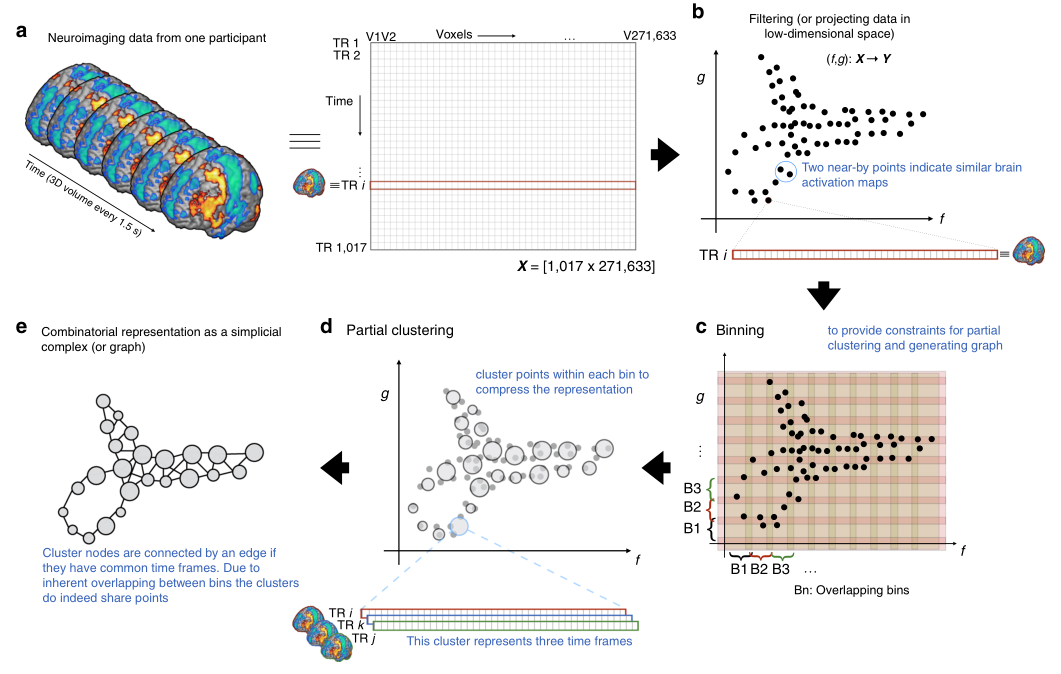
\includegraphics[width = 0.75\linewidth]{fig1.png}
        \caption{The method used to convert the 4-dimensional fMRI data into a simplicial complex. Steps b-e are a part of Mapper (the TDA-based algorithm/tool the authors used).}
    \end{figure}
\end{frame}

\begin{frame}{How Mapper works}
    \begin{itemize}
        \item Step 1 the filtering into $\R^2$ is done using something called Stochastic Neighborhood Estimation. SNE, is used over traditional methods like PCA because SNE allows us to preserve the local structure of the original data \pause % PCA involves changing basis and thus destroys local structure
        \item Step 2 is just binning the space using the provided parameters: number of bins and the percentage overlap between bins\pause
        \item Step 3 goes through each bin, and performs single-linkage clustering in order to form clusters of nearby points\pause 
        \item Step 4 treats each cluster as a vertex of a graph and adds an edge between two vertices if they shared a point\cite{mapper}
        % The authors used something called the CMP dataset which is pretty standard and after applying mapper to each participant in CMP, they want to analyze the properties of each person's graph
    \end{itemize}
\end{frame}

\begin{frame}{Filtering in Mapper}
    \begin{figure}
        \begin{columns}
            \begin{column}{0.4\textwidth}
                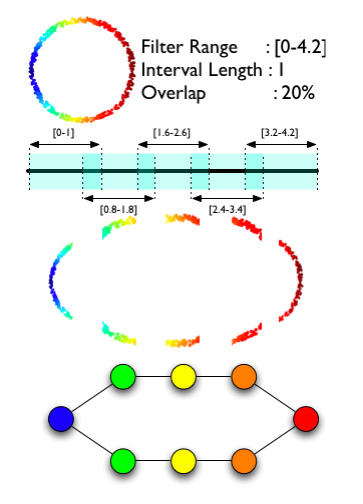
\includegraphics[width = \linewidth]{filter.png}
            \end{column}
            \begin{column}{0.55\textwidth}
                \caption{Toy example of applying a filter to data\cite{mapper}. The data is sampled from a noisy circle, and the filter used is $f(x) = ||x - p||^2$, where $p$ is the left most point in the data. We divide the range of the filter into 5 intervals which have length 1 and a 20$\%$ overlap. For each interval we compute the clustering of the points lying within the domain of the filter restricted to the interval, and connect the clusters whenever they have non-empty intersection. At the bottom is the simplicial complex which we recover whose vertices are colored by the average filter value.}
            \end{column}
        \end{columns}
    \end{figure}
\end{frame}

\begin{frame}{Diagram of the Filtering process}
    \begin{figure}
        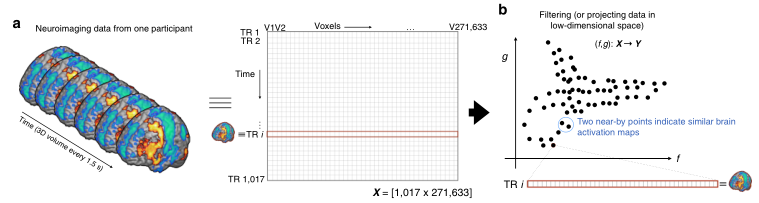
\includegraphics[width = 0.9\linewidth]{fig1ab.png}
        \caption{Our paper uses a very different filter function than the previous example. They use something called the Neighborhood Lens function to take their 271633-dimensional data into $\R^2$. This function is part of a patented software that appears to be standard.}
    \end{figure}
\end{frame}

\begin{frame}{Clustering}
    \begin{figure}
        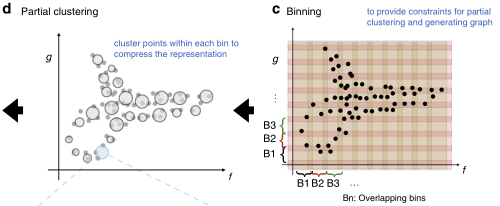
\includegraphics[width=0.8\linewidth]{fig1cd.png}
        \caption{Mapper take two parameters when binning the data: Resolution and Gain. Resolution controls the number of bins and Gain controls the overlap between bins.}
    \end{figure}
\end{frame}

\begin{frame}{Example}
    \begin{figure}
        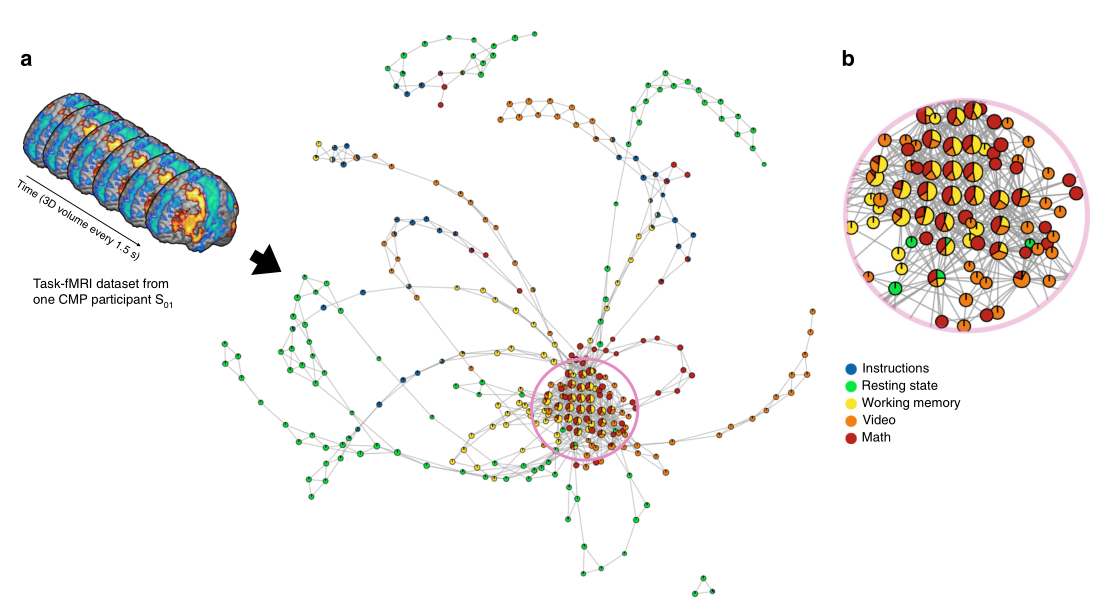
\includegraphics[width = 0.85\linewidth]{fig2.png}
        \caption{After running Mapper on an individual's fMRI data, we are left with a graph like the above. The fMRI datasets ($1017\times271633)$ matrix) were compressed to $279\pm60$ points.}
    \end{figure}
\end{frame}

\begin{frame}{How do we analyze these graphs?}
    \begin{itemize}
        \item The most interesting and practical thing we can do with this graph is try to understand the mesoscale structure of this graph \pause
        \item The most commonly analyzed mesoscale structures are community structures and core-periphery structures \pause
        \item Note: It is necessary to have weights on the edges to perform analysis of community structure or core-periphery structure
        \item This paper doesn't describe how they acquire weights on the edges and there is no canonical way to assign weights from mapper \pause
        \item Two likely possibilities: the weight between two nodes is the number of timeframes they shared, or the weight is something that depends on the mean distance between the timeframes constituting the nodes
    \end{itemize}
\end{frame}

\begin{frame}{Analyzing the community structure of a graph}
    \begin{itemize}
        \item You can think about the community structure as the measure of if there are many ``communities'' of densely connected nodes (not necessarily cliques) there are where there are only a few connections between communities \pause
        \item Suppose that you have a weighted graph $G$ and for each vertex $i$, we have ``node strength" weight $k_i$ on $i$ \pause
        \item $Q_{\mathrm{mod}}$ (called the modularity) is the most commonly used metric to assess the community structure of a graph\cite{community} \pause
    \end{itemize}
    \[Q_{\mathrm{mod}} = \sum_{i,j} \left(A_{ij} - P_{ij}\right)\delta(g_i, g_j)\]
    where $A$ is the adjacency matrix, $P_{ij} = \frac{k_i k_j}{\sum_{ij}A_{ij}}$, $k_i$ is degree of $i$, $g_i$ is the community that $i$ belongs to, and $\delta$ is the Kronecker delta.
\end{frame}

\begin{frame}{Some intuition for $Q_{\mathrm{mod}}$}
    \begin{itemize}
        \item It is based on the idea that a random graph is not expected to have a cluster structure, so the possible existence of clusters is revealed by the comparison between the actual density of edges in a subgraph and the density one would expect to have in the subgraph if the vertices of the graph
        were attached regardless of community structure
        \item This expected edge density ($P_{ij} = \frac{k_ik_j}{2m}$ where $m = \sum_{ij}A_{ij}$) depends on the chosen null model, i.e. a copy of the original graph keeping some of its structural properties but without community structure\cite{community}\pause
        \item In this case, the null model that produces the above expected edge density is called the configuration model. This a very standard type of model in network science because, as opposed to the Erd\H{o}s-Renyi model, this model allows us to give the network arbitrary degree distributions. (The Erd\H{o}s-Renyi model only allows for Poisson distribution for the degree sequence).
    \end{itemize}
\end{frame}

\begin{frame}{How $Q_{\mathrm{mod}}$ scales}
    \begin{figure}
        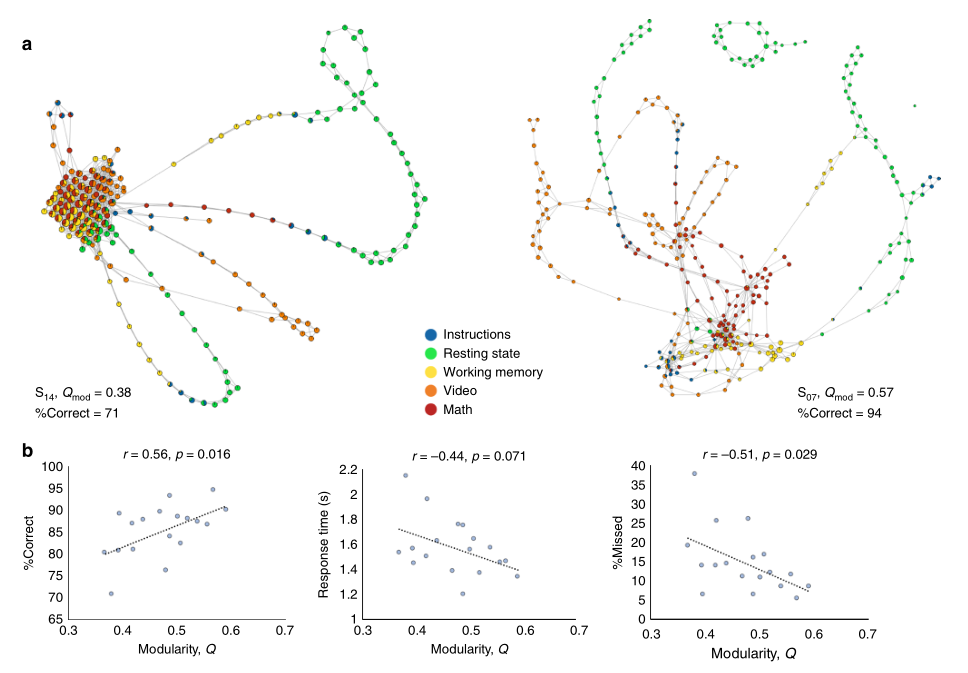
\includegraphics[width = 0.75\linewidth]{fig3.png}
        \caption{There are two different participants' shape graphs and the relations between modularity and various metrics}
    \end{figure}
\end{frame}

\begin{frame}{Analyzing the core-periphery structure of the graph}
    \begin{itemize}
        \item We assign each node a coreness score (CS) by giving higher scores to nodes which lie deeper in the network
        \item The Borgatti-Everett algorithm is an algorithm that assigns coreness scores to each vertex of the shape graph. If we call $C_i$ is the coreness of vertex $i$, then we can define the core matrix $C$ by $C_{ij} = C_{i}C_j$. We can define a quality function \[R_{(\alpha,\beta)} = \sum_{i,j}A_{ij}C_{ij}\]where $(\alpha, \beta)$ are the two parameters which determines the boundary between the core and periphery and size of the core respectively. A large $\alpha$ indicates a sharp transition
    \end{itemize}
\end{frame}

\begin{frame}{Definition of the aggregate of coreness scores}
    Recall that 
    \[R_{(\alpha,\beta)} = \sum_{i,j}A_{ij}C_{ij}\]
    The aggregate of coreness of node $i$ is \[CS(i) = Z \sum_{(\alpha, \beta)} C_i(\alpha, \beta) \times R(\alpha, \beta)\]where $Z$ is a normalization factor to make the maximum $CS$ be 1 and this sum is not actually over all $\alpha,\beta$ but instead over a uniform sampling of a discretization of the unit square.
\end{frame}

\begin{frame}{How coreness score (CS) scales}
    \begin{figure}
        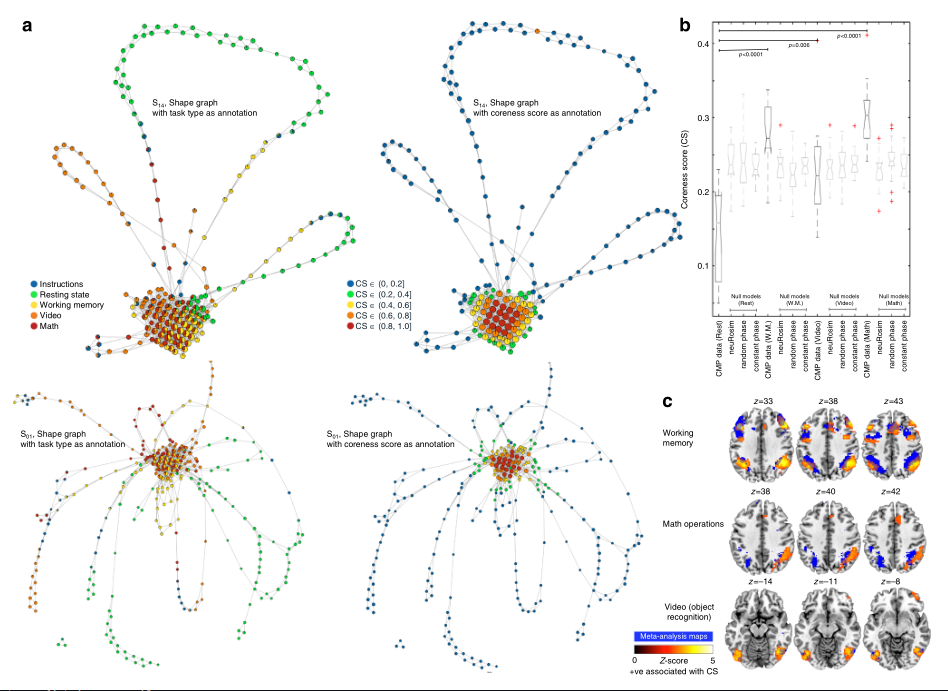
\includegraphics[width = 0.85\linewidth]{fig4.png}
        %\caption{CS for two different shape graphs, CS derived from our data and some null models, and a diagram of regions of the brain that were associated with high coreness}
    \end{figure}
\end{frame}

\begin{frame}{Trying to explain the topological features using anatomy}
    \begin{itemize}
        \item 
    \end{itemize}
\end{frame}

\begin{frame}{Connectivity in the shape graph for different times}
    \begin{figure}
        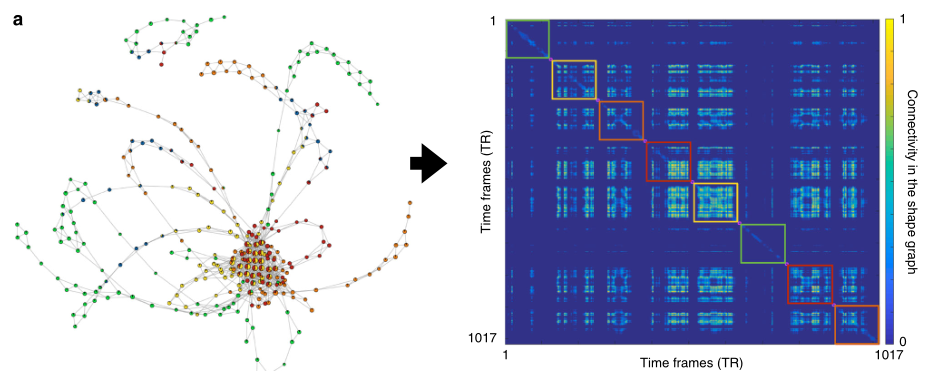
\includegraphics[width = 0.95\linewidth]{fig5a.png}
        \caption{Shows which times during the scan were similar to other times by looking at the connections between times in the shape graph.}
    \end{figure}
\end{frame}

\begin{frame}{Brains are typically more connected during strenuous tasks}
    \begin{figure}
        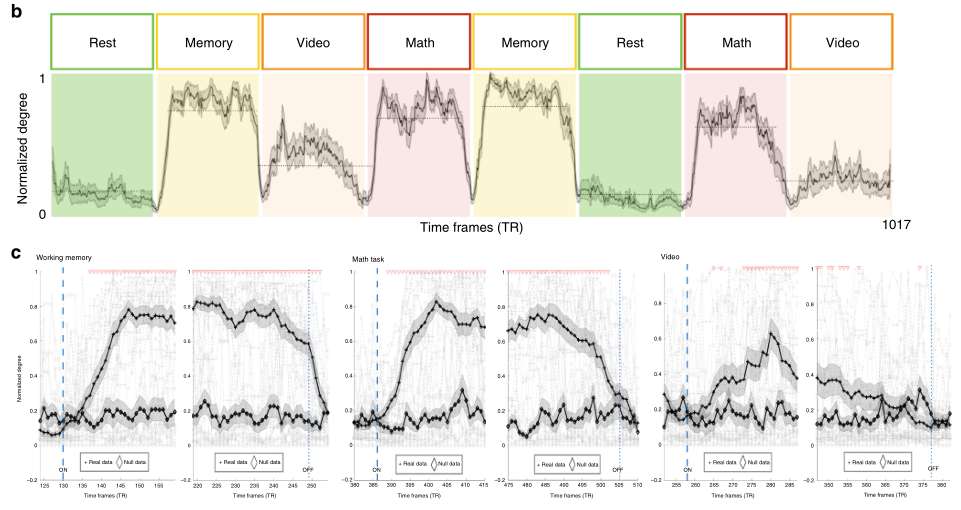
\includegraphics[width = 0.85\linewidth]{fig5b.png}
        \caption{When there is a transition between tasks, this is captured by a dramatic change in the degree of the corresponding nodes. This phenomenon of nodes taken during strenuous activity having high degree is significant}
    \end{figure}
\end{frame}

\begin{frame}{}
    
\end{frame}

\begin{frame}{}
    
\end{frame}

\begin{frame}[allowframebreaks]{References}
\printbibliography
\end{frame}

% %------------------------------------------------

\begin{frame}
\Huge{\centerline{The End}}
\end{frame}

%----------------------------------------------------------------------------------------

\end{document} 